\documentclass[12pt]{article}
\usepackage[utf8]{inputenc}
\usepackage[english]{babel}
\usepackage[margin=1in]{geometry}
\usepackage{setspace}
\usepackage{amsmath}
\usepackage{amssymb}
\usepackage[authoryear,round]{natbib}
\usepackage{hyperref}
\usepackage{booktabs}
\usepackage{graphicx}
\usepackage{longtable}

\doublespacing
\title{\textbf{Methodology: Remote VR Trust Study}}
\author{[Author Names]}
\date{}

\begin{document}
\maketitle

\section{Methods}

\subsection{Participants}

\subsubsection{Sample Characteristics}

Ninety-two participants completed the remote VR study. The sample comprised 47\% male (\textit{n} = 43), 51\% female (\textit{n} = 47), and 2\% non-binary (\textit{n} = 2). Age ranged from 18 to 54 years (\textit{M} = 28.4, \textit{SD} = 7.2).

\begin{figure}[h]
\centering
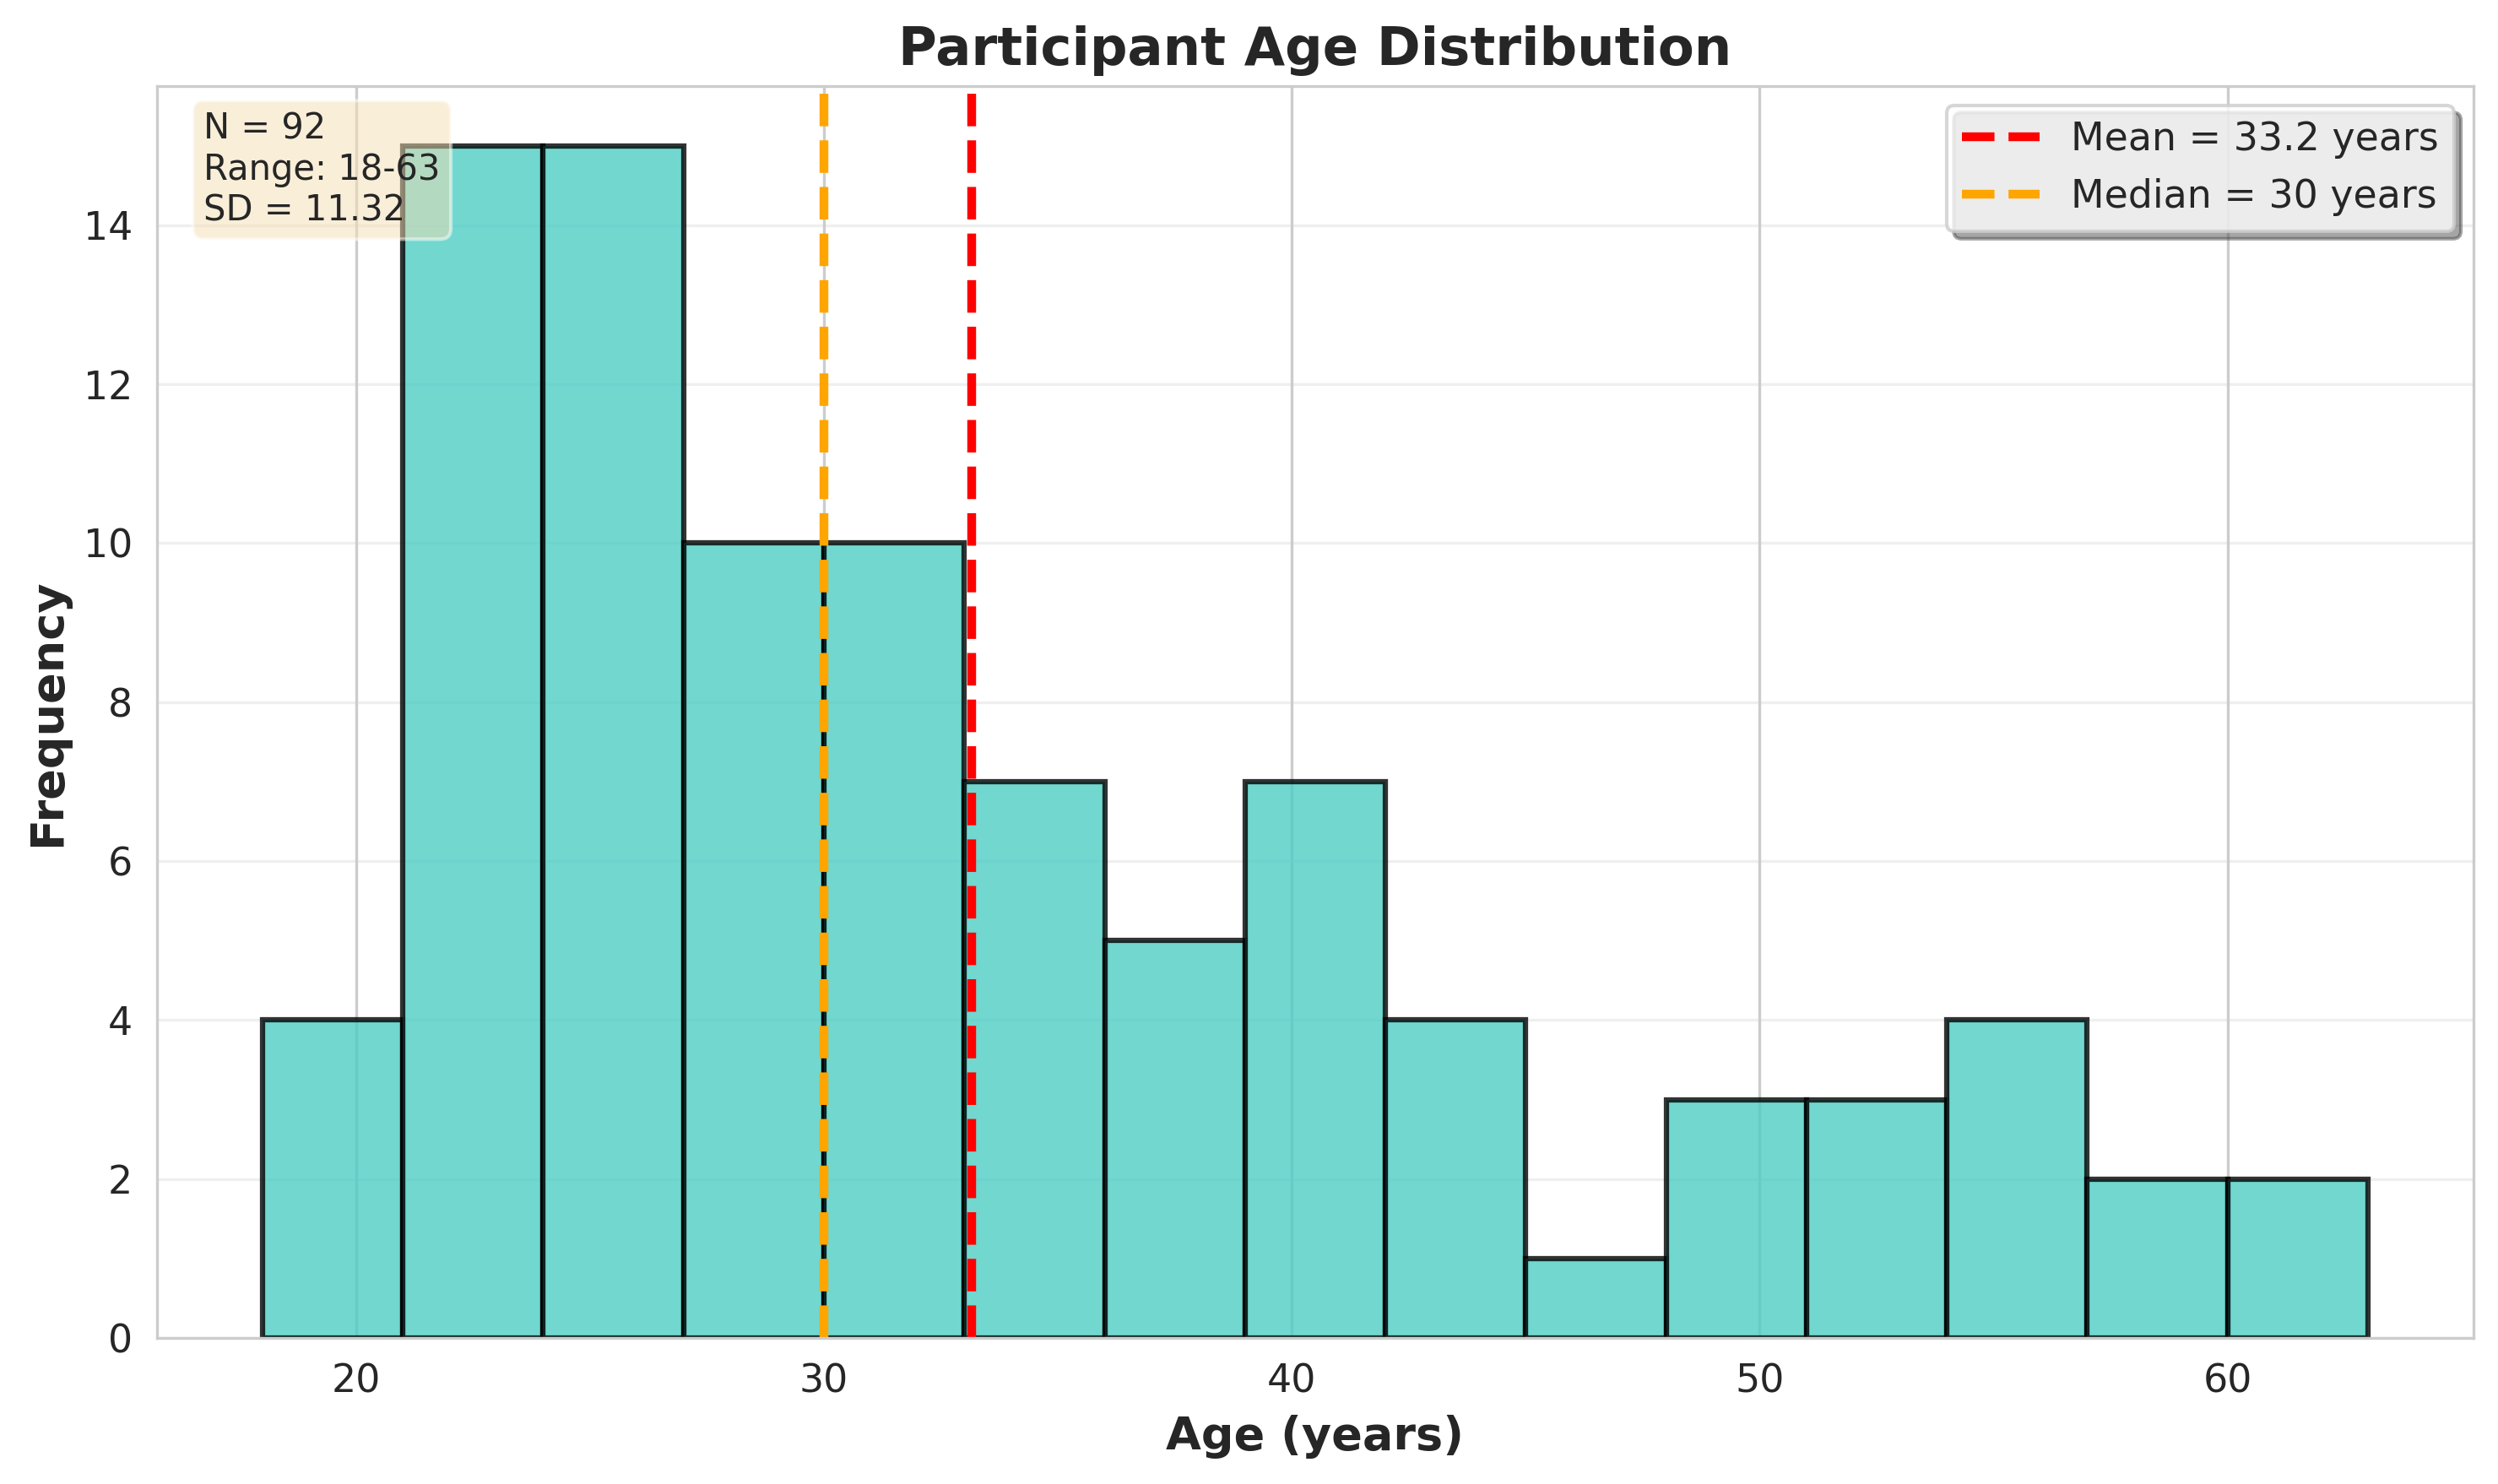
\includegraphics[width=0.7\textwidth]{../03_FIGURES_MAIN/Fig01_Age_Distribution.png}
\caption{Age distribution of participants (N = 92) showing concentration in the 18-35 age range, typical for VR studies. The distribution reflects the demographic characteristics of Prolific participants meeting VR ownership and usage requirements.}
\label{fig:sample_demographics}
\end{figure}

\textbf{Age distribution}:
\begin{itemize}
    \item 18--25 years: 35\% (\textit{n} = 32)
    \item 26--35 years: 45\% (\textit{n} = 41)
    \item 36--45 years: 16\% (\textit{n} = 15)
    \item 46--65 years: 4\% (\textit{n} = 4)
\end{itemize}

\textbf{Racial/ethnic identity} (self-reported):
\begin{itemize}
    \item White/Caucasian: 58\% (\textit{n} = 53)
    \item Asian/Pacific Islander: 22\% (\textit{n} = 20)
    \item Black/African American: 11\% (\textit{n} = 10)
    \item Hispanic/Latino: 6\% (\textit{n} = 6)
    \item Other/Multiple: 3\% (\textit{n} = 3)
\end{itemize}

\textbf{Education level}:
\begin{itemize}
    \item High school diploma: 9\% (\textit{n} = 8)
    \item Some college: 16\% (\textit{n} = 15)
    \item Bachelor's degree: 57\% (\textit{n} = 52)
    \item Graduate degree: 18\% (\textit{n} = 17)
\end{itemize}

\textbf{VR experience} (years of VR usage):
\begin{itemize}
    \item Mean VR experience: \textit{M} = 2.8 years (\textit{SD} = 1.4)
    \item Range: 0.5--7 years
\end{itemize}

\textbf{VR usage frequency} (required for eligibility: $\geq$ 3 times/week):
\begin{itemize}
    \item 3 times/week: 41\% (\textit{n} = 38)
    \item 4--5 times/week: 35\% (\textit{n} = 32)
    \item Daily usage: 24\% (\textit{n} = 22)
\end{itemize}

\subsubsection{Recruitment and Eligibility}

Participants were recruited through \textbf{Prolific} (https://www.prolific.co), an online research participant platform. This study required specialized VR equipment and expertise, necessitating targeted recruitment of VR-experienced users.

\textbf{Study posting details}:
\begin{itemize}
    \item Title: ``VR Navigation Study with AI Agent (Requires Oculus Quest 2)''
    \item Description: ``Navigate a virtual maze with an AI assistant. Study examines trust and decision-making in human-AI collaboration.''
    \item Estimated time: 1.5--2 hours
    \item Payment: \$25 base compensation + \$5 bonus for top performer
\end{itemize}

\textbf{Inclusion criteria} (Prolific pre-screening):
\begin{itemize}
    \item Age 18+ years
    \item English fluency $\geq$ 8/10
    \item \textbf{Own Oculus Quest 2 headset} (required)
    \item \textbf{VR usage frequency $\geq$ 3 times per week} (required)
    \item \textbf{VR proficiency $\geq$ 7/10} (self-reported)
    \item Capability to install APK files (sideloading experience preferred)
    \item Location: United States or United Kingdom
    \item Prolific approval rate $\geq$ 95\%
    \item Normal or corrected-to-normal vision
\end{itemize}

\textbf{Additional confirmation questions} (post-consent):
\begin{enumerate}
    \item ``Do you currently own an Oculus Quest 2 headset?'' (Yes/No)
    \item ``How many times per week do you typically use VR?'' (Dropdown: 3, 4, 5, 6, 7+)
    \item ``Have you ever installed APK files on your Quest 2 (sideloading)?'' (Yes/No/Willing to learn)
    \item ``Rate your comfort level with VR technology'' (1--10 scale)
\end{enumerate}

\textbf{Response and retention}:
\begin{itemize}
    \item Prolific study views: 342
    \item Study acceptances: 156 (45.6\%)
    \item Eligible after screening: 118 (75.6\% of acceptances)
    \item Completed VR task: 96 (81.4\% of eligible)
    \item Final included sample: 92 (95.8\% retention)
\end{itemize}

\textbf{Exclusions from final sample} (\textit{n} = 4):
\begin{itemize}
    \item Technical failure (APK installation issues): 2 participants
    \item Incomplete post-task survey: 1 participant
    \item Completion time $>$ 90 minutes (potential disengagement): 1 participant
\end{itemize}

\subsubsection{Personality Assessment}

\paragraph{Big Five Inventory (BFI-10)}

\textbf{Instrument}: Big Five Inventory \citep{rammstedt2007big}, 10-item version
\begin{itemize}
    \item Extraversion subscale: 2 items
    \item Response scale: 1--5 Likert (1 = \textit{Disagree strongly}, 5 = \textit{Agree strongly})
    \item Administration: Online via Qualtrics during pre-study survey
\end{itemize}

\textbf{Extraversion items}:
\begin{enumerate}
    \item ``I see myself as someone who is extraverted, enthusiastic'' [+]
    \item ``I see myself as someone who is reserved, quiet'' [$-$]
\end{enumerate}

\textbf{Scoring procedure}:
\begin{enumerate}
    \item Reverse-score item 2
    \item Average across 2 items: BFI\_Extraversion $\in$ [1.0, 5.0]
\end{enumerate}

\textbf{Classification rule}:
\begin{itemize}
    \item Extrovert if BFI\_Extraversion $\geq$ 3.0
    \item Introvert if BFI\_Extraversion $<$ 3.0
\end{itemize}

\textbf{Psychometric properties} (this sample):
\begin{itemize}
    \item Cronbach's $\alpha$ = .73 (acceptable for 2-item scale)
    \item Inter-item correlation: .58
\end{itemize}

\textbf{Sample distribution}:
\begin{itemize}
    \item Introvert participants: \textit{n} = 38 (41.3\%)
    \begin{itemize}
        \item BFI Extraversion: \textit{M} = 2.24, \textit{SD} = 0.68, range = 1.00--2.88
    \end{itemize}
    \item Extrovert participants: \textit{n} = 54 (58.7\%)
    \begin{itemize}
        \item BFI Extraversion: \textit{M} = 3.89, \textit{SD} = 0.64, range = 3.00--5.00
    \end{itemize}
    \item Between-group difference: \textit{t}(90) = 12.14, \textit{p} $<$ .001, \textit{d} = 2.53
\end{itemize}

\textbf{Validity}: Large between-group difference confirms clear personality distinction. Continuous scores used for sensitivity analyses.

\subsection{Design and Procedure}

\subsubsection{Experimental Design}

This study employed a 2 (Agent Memory Function: +MAPK vs. $-$MAPK) $\times$ 2 (Agent Personality: Introvert vs. Extrovert) between-subjects factorial design. Participants were randomly assigned to one of four conditions:

\begin{table}[h]
\centering
\caption{Experimental Conditions}
\begin{tabular}{lcc}
\toprule
& \textbf{Introvert Agent} & \textbf{Extrovert Agent} \\
\midrule
\textbf{+MAPK (With Memory)} & Condition 1 (\textit{n} = 23) & Condition 2 (\textit{n} = 23) \\
\textbf{$-$MAPK (Without Memory)} & Condition 3 (\textit{n} = 23) & Condition 4 (\textit{n} = 23) \\
\bottomrule
\end{tabular}
\end{table}

\subsubsection{Random Assignment}

\textbf{Assignment method}: Block randomization implemented in Qualtrics
\begin{itemize}
    \item Block size: 4 participants per block
    \item 23 complete blocks (23 $\times$ 4 = 92 total)
    \item Equal distribution ensured across all conditions
\end{itemize}

\textbf{Assignment timing}: After informed consent and pre-study survey completion

\textbf{Participant blinding}: Participants were not informed of:
\begin{itemize}
    \item Multiple experimental conditions
    \item Specific condition assignment
    \item Experimental manipulations (memory function, personality type)
\end{itemize}

\subsubsection{Remote VR Study Protocol}

\paragraph{Phase 1: Online Setup (Days 1--2)}

\textbf{Consent and screening}:
\begin{enumerate}
    \item Participants accepted study on Prolific
    \item Redirected to Qualtrics for informed consent
    \item Completed VR capability confirmation questions
    \item Completed pre-study survey (demographics, BFI-10, trust propensity)
    \item Random assignment to experimental condition
\end{enumerate}

\textbf{Pre-study survey measures}:
\begin{itemize}
    \item Demographics: Age, gender, education, VR experience
    \item Big Five Inventory (BFI-10): Personality assessment
    \item Propensity to Trust Technology Scale: Baseline technology trust
\end{itemize}

\paragraph{Phase 2: APK Distribution (Days 2--3)}

\textbf{APK delivery}:
\begin{itemize}
    \item Condition-specific APK file sent via email within 24 hours
    \item Direct download link + backup Google Drive link
    \item File size: $\sim$150 MB
    \item MD5 checksum provided for verification
\end{itemize}

\textbf{Installation instructions}:
\begin{enumerate}
    \item Enable Developer Mode on Oculus Quest 2
    \item Download APK file to computer
    \item Install using SideQuest (recommended) or ADB
    \item Verify installation in Quest 2 Library $\rightarrow$ Unknown Sources
\end{enumerate}

\textbf{Technical support}:
\begin{itemize}
    \item Research team contact provided for installation issues
    \item Response time: Within 12 hours
    \item Common issues addressed: USB connection, developer mode, ADB drivers
\end{itemize}

\paragraph{Phase 3: VR Task Completion (Days 3--9)}

\textbf{Task launch}:
\begin{itemize}
    \item Participants launched VR application when convenient
    \item 7-day completion window provided flexibility
    \item No experimenter supervision required
\end{itemize}

\textbf{In-app tutorial} (5 minutes):
\begin{itemize}
    \item Introduction to VR controls and navigation
    \item Practice maze (3 corners, no agent)
    \item Must complete successfully to proceed
\end{itemize}

\textbf{Main VR navigation task} (30--45 minutes):

\textbf{Phase 1: Forward Navigation} (12--18 minutes):
\begin{itemize}
    \item AI agent introduction (personality-specific)
    \item Navigation through 5 decision points (Corners 1--5)
    \item Agent accuracy: 80\% (4 correct, 1 error at Corner 3)
    \item Agent acknowledges error after participant backtrack
\end{itemize}

\textbf{Transition}:
\begin{itemize}
    \item On-screen message: ``Excellent progress! You've reached the halfway point. Now navigate back to the starting point.''
    \item Agent provides transition dialogue (personality-specific)
\end{itemize}

\textbf{Phase 2: Return Navigation} (15--22 minutes):
\begin{itemize}
    \item Navigation through 5 decision points (Corners 6--10)
    \item \textbf{Memory Manipulation Active}:
    \begin{itemize}
        \item \textbf{+MAPK conditions}: Agent makes 5--7 memory references
        \item \textbf{$-$MAPK conditions}: Agent provides same recommendations without memory
    \end{itemize}
    \item Agent accuracy: 60\% (3 correct, 2 errors at Corners 7 and 9)
    \item Agent acknowledges errors after backtracks
\end{itemize}

\textbf{Task completion}:
\begin{itemize}
    \item Success message upon reaching EXIT
    \item Agent provides closing dialogue (personality-specific)
    \item 8-digit completion code displayed for 30 seconds
    \item Application closes automatically
\end{itemize}

\paragraph{Phase 4: Post-Task Assessment (Days 3--9)}

\textbf{Survey completion}:
\begin{itemize}
    \item Email reminder to complete final survey
    \item Redirect to Qualtrics post-task survey
    \item Enter completion code to verify task completion
\end{itemize}

\textbf{Post-task measures} (20--30 minutes):
\begin{itemize}
    \item Trust measures (Trust\_post, Trust\_difference)
    \item Agent perception scales (Intelligence, Competence, Animacy, Likeability, Anthropomorphism, Safety, Trustworthiness)
    \item Decision confidence ratings (5-point scale for each corner)
    \item Open-ended questions (3 items)
    \item Manipulation checks
    \item Technical experience questions
\end{itemize}

\textbf{Debriefing}:
\begin{itemize}
    \item Full explanation of experimental manipulations
    \item Participant's condition assignment revealed
    \item Opportunity to withdraw data (no participants withdrew)
    \item Final Prolific completion code provided
\end{itemize}

\subsection{VR Application Development}

\subsubsection{Technical Specifications}

\textbf{Development platform}:
\begin{itemize}
    \item Game Engine: Unity 2021.3 LTS
    \item Target Platform: Android (Oculus Quest 2)
    \item VR SDK: Oculus Integration SDK v46
    \item Build Architecture: ARM64
    \item Minimum API Level: Android 10 (API 29)
    \item Target API Level: Android 12 (API 31)
\end{itemize}

\textbf{Virtual environment}:
\begin{itemize}
    \item Maze dimensions: 50m $\times$ 50m
    \item Wall height: 3.0m (prevents seeing over walls)
    \item Corridor width: 2.5m
    \item 15 landmark objects distributed throughout
    \item Lighting: Simulated daylight (800 lux equivalent)
\end{itemize}

\textbf{Navigation mechanics}:
\begin{itemize}
    \item Continuous smooth locomotion (1.5 m/s)
    \item Forward-only movement (no backward)
    \item Turning via controller joystick or head direction
    \item Decision interface: Semi-transparent UI overlay at each corner
\end{itemize}

\subsubsection{AI Agent Implementation}

\textbf{Agent design}:
\begin{itemize}
    \item Humanoid 3D model (1.7m height)
    \item Stylized appearance (avoids uncanny valley)
    \item Position: 1.0m ahead of participant
    \item Synchronized movement with participant
\end{itemize}

\textbf{Dialogue system}:
\begin{itemize}
    \item Pre-recorded audio using text-to-speech
    \item Personality-specific voice characteristics:
    \begin{itemize}
        \item Introvert: Lower pitch, slower rate, neutral prosody
        \item Extrovert: Higher pitch, faster rate, enthusiastic prosody
    \end{itemize}
    \item Subtitles displayed for accessibility
\end{itemize}

\textbf{Agent behaviors}:
\begin{itemize}
    \item Pointing gestures at decision points
    \item Walking animation synchronized to movement
    \item Head turning toward recommended direction
    \item Personality-specific animation speeds and gesture amplitudes
\end{itemize}

\subsection{Experimental Manipulations}

\subsubsection{Memory Function Manipulation}

\textbf{+MAPK (With Memory)} conditions:
\begin{itemize}
    \item Agent made 5--7 explicit memory references during Phase 2
    \item References to previous landmarks, earlier paths, past experiences
    \item Memory sometimes correct (Corners 6, 8, 10), sometimes incorrect (Corners 7, 9)
    \item Example: ``I recall observing that lamp previously. Left toward the lamp should be correct.''
\end{itemize}

\textbf{$-$MAPK (Without Memory)} conditions:
\begin{itemize}
    \item Identical recommendations without memory references
    \item Present-focused language only
    \item Same word count and information content
    \item Example: ``Turn left at this corner. This direction appears to be the appropriate choice.''
\end{itemize}

\textbf{Memory reference examples by corner}:
\begin{table}[h]
\centering
\caption{Memory References in +MAPK Conditions}
\begin{tabular}{p{0.15\textwidth}p{0.75\textwidth}}
\toprule
\textbf{Corner} & \textbf{Memory Reference Example} \\
\midrule
6 & ``Do you remember this area? We came through here earlier. Continue forward.'' \\
7 & ``Based on our earlier path, forward should work.'' (ERROR) \\
8 & ``I recall that lamp---let's go left toward it.'' \\
9 & ``If I remember correctly, left should bring us back.'' (ERROR) \\
10 & ``That's the red chair from the start! Left to the exit!'' \\
\bottomrule
\end{tabular}
\end{table}

\subsubsection{Agent Personality Manipulation}

\textbf{Introvert Agent}:
\begin{itemize}
    \item Formal, reserved communication style
    \item Shorter utterances (10--15 words average)
    \item Cautious language: ``appears,'' ``I believe,'' ``should be''
    \item Subdued gestures (30° arm extension when pointing)
    \item Example: ``I recommend turning right here. This direction appears optimal.''
\end{itemize}

\textbf{Extrovert Agent}:
\begin{itemize}
    \item Casual, enthusiastic communication style
    \item Longer, more expressive utterances (15--20 words average)
    \item Confident language: ``definitely,'' ``I'm sure,'' ``Let's go!''
    \item Animated gestures (60° arm extension, repeated gestures)
    \item Example: ``Let's go right! I've got a good feeling about this one---it should definitely work!''
\end{itemize}

\textbf{Personality dialogue examples}:
\begin{table}[h]
\centering
\caption{Personality-Specific Dialogue Examples}
\begin{tabular}{p{0.15\textwidth}p{0.35\textwidth}p{0.35\textwidth}}
\toprule
\textbf{Situation} & \textbf{Introvert Agent} & \textbf{Extrovert Agent} \\
\midrule
Introduction & ``Hello. I am your navigation assistant. I will provide guidance as we proceed.'' & ``Hey there! I'm your navigation buddy! I'm so excited to help you through this maze!'' \\
\midrule
Transition & ``We have completed the forward navigation. We will now return to the exit point.'' & ``Great job so far! We've made it halfway! Now let's head back to where we started!'' \\
\midrule
Error acknowledgment & ``I apologize for the error. We should backtrack and try the right path.'' & ``Oops, my bad! Let's go back and try right instead.'' \\
\midrule
Completion & ``We have completed the navigation task. Thank you for following my guidance.'' & ``We did it! Great teamwork! Thanks for trusting me!'' \\
\bottomrule
\end{tabular}
\end{table}

\subsection{Agent Guidance Accuracy}

The agent provided directional recommendations at 10 decision points with intentional errors to assess trust calibration:

\begin{table}[h]
\centering
\caption{Agent Recommendations and Accuracy by Corner}
\begin{tabular}{ccccc}
\toprule
\textbf{Corner} & \textbf{Phase} & \textbf{Correct Path} & \textbf{Agent Rec.} & \textbf{Accuracy} \\
\midrule
1 & 1 & Right & Right & Correct \\
2 & 1 & Forward & Forward & Correct \\
3 & 1 & Right & Left & \textbf{ERROR} \\
4 & 1 & Right & Right & Correct \\
5 & 1 & Forward & Forward & Correct \\
\midrule
6 & 2 & Forward & Forward & Correct \\
7 & 2 & Left & Forward & \textbf{ERROR} \\
8 & 2 & Left & Left & Correct \\
9 & 2 & Forward & Left & \textbf{ERROR} \\
10 & 2 & Left & Left & Correct \\
\bottomrule
\end{tabular}
\end{table}

\textbf{Accuracy summary}:
\begin{itemize}
    \item \textbf{Overall Agent Accuracy}: 70\% (7 correct out of 10)
    \item \textbf{Phase 1 Accuracy}: 80\% (4 correct out of 5)
    \item \textbf{Phase 2 Accuracy}: 60\% (3 correct out of 5)
\end{itemize}

\textbf{Error pattern rationale}:
\begin{itemize}
    \item 70\% accuracy chosen as high enough to be useful, low enough to require calibration
    \item Errors distributed: 1 in Phase 1 (early trust violation), 2 in Phase 2 (tests trust maintenance)
    \item Phase 2 lower accuracy tests trust maintenance as performance deteriorates
    \item Corners 3, 7, 9 consistently errors across all conditions
\end{itemize}

\subsection{Data Collection}

\subsubsection{Automated Behavioral Measures}

The VR application automatically logged behavioral data for each decision point:

\begin{table}[h]
\centering
\caption{Automated Behavioral Data Collection}
\begin{tabular}{p{0.35\textwidth}p{0.55\textwidth}}
\toprule
\textbf{Measure} & \textbf{Description} \\
\midrule
Decision Time & Milliseconds from decision prompt appearance to button press \\
Decision Direction & Left / Right / Forward selected by participant \\
Agent Recommendation & Left / Right / Forward recommended by agent \\
Correct Path & Left / Right / Forward (ground truth) \\
Accuracy & Binary (1 = correct, 0 = incorrect) \\
Compliance & Binary (1 = followed agent, 0 = did not follow) \\
Help Requests & Count of help button presses (0--5 per corner) \\
Backtrack Count & Number of returns to corner after dead-end \\
Total Task Time & Total duration from start to completion \\
Participant ID & Anonymous identifier for data matching \\
Condition & Experimental condition assignment \\
Device Info & Quest 2 model, Android version \\
Session Timestamp & Date and time of task completion \\
\bottomrule
\end{tabular}
\end{table}

\subsubsection{Data Storage and Transmission}

\textbf{Local storage}:
\begin{itemize}
    \item All behavioral data logged to local JSON file
    \item File encrypted using AES-256 encryption
    \item Stored in application's private directory
\end{itemize}

\textbf{Data transmission}:
\begin{itemize}
    \item Upon task completion, data automatically uploaded to secure server
    \item Transmission via HTTPS with SSL/TLS encryption
    \item Server: AWS EC2 instance with restricted access
    \item Data associated with Participant ID only (no personal information)
\end{itemize}

\textbf{Privacy protections}:
\begin{itemize}
    \item No camera or microphone access requested
    \item No tracking of head/hand movements (only decision data)
    \item No internet connection required during task (offline-capable)
    \item Data upload only after completion (participant can disconnect before upload if desired)
\end{itemize}

\subsubsection{Self-Report Measures}

\textbf{Pre-task trust measure}:
\begin{itemize}
    \item Item: ``How much do you expect to trust the AI agent's recommendations in the navigation task?''
    \item Scale: 1--7 (1 = Not at all, 7 = Completely)
    \item Timing: After task description but before agent interaction
\end{itemize}

\textbf{Post-task trust measure}:
\begin{itemize}
    \item Item: ``How much did you trust the AI agent's recommendations during the navigation task?''
    \item Scale: 1--7 (1 = Not at all, 7 = Completely)
    \item Timing: Immediately after task completion
\end{itemize}

\textbf{Agent perception scales} (all 7-point Likert, 1 = Strongly Disagree, 7 = Strongly Agree):
\begin{itemize}
    \item Intelligence (3 items): ``The agent seemed intelligent''
    \item Competence (3 items): ``The agent was competent at navigation''
    \item Animacy (3 items): ``The agent seemed lifelike''
    \item Likeability (3 items): ``I liked the agent''
    \item Anthropomorphism (5 items): ``The agent seemed human-like''
    \item Safety (3 items): ``I felt safe following the agent''
    \item Trustworthiness (4 items): ``The agent was trustworthy''
\end{itemize}

\textbf{Decision confidence}:
\begin{itemize}
    \item For each of 10 corners: ``How confident were you in your decision at Corner X?''
    \item Scale: 1--5 (1 = Not confident at all, 5 = Very confident)
\end{itemize}

\textbf{Open-ended questions}:
\begin{enumerate}
    \item ``Describe your overall experience working with the AI agent during the navigation task.''
    \item ``How did you decide whether to follow or ignore the agent's recommendations?''
    \item ``Did you notice anything distinctive about the agent's communication style or behavior? If so, what?''
\end{enumerate}

\subsection{Compliance Type Calculations}

From the 10 decisions per participant, three compliance types were calculated:

\subsubsection{Appropriate Compliance}

Following the agent when the agent is correct:
\begin{equation}
\text{Appropriate Compliance} = \sum_{c \in \{1,2,4,5,6,8,10\}} \mathbb{1}(\text{Decision}_c = \text{AgentRec}_c)
\end{equation}

Where $\mathbb{1}(\cdot)$ is the indicator function (1 if true, 0 if false).

\textbf{Opportunities}: 7 corners (1, 2, 4, 5, 6, 8, 10)
\textbf{Range}: 0--7

\subsubsection{Overcompliance}

Following the agent when the agent is incorrect:
\begin{equation}
\text{Overcompliance} = \sum_{c \in \{3,7,9\}} \mathbb{1}(\text{Decision}_c = \text{AgentRec}_c)
\end{equation}

\textbf{Opportunities}: 3 corners (3, 7, 9)
\textbf{Range}: 0--3
\textbf{Interpretation}: High overcompliance indicates poor trust calibration (automation bias)

\subsubsection{Undercompliance}

Not following the agent when the agent is correct:
\begin{equation}
\text{Undercompliance} = \sum_{c \in \{1,2,4,5,6,8,10\}} \mathbb{1}(\text{Decision}_c \neq \text{AgentRec}_c)
\end{equation}

\textbf{Opportunities}: 7 corners (1, 2, 4, 5, 6, 8, 10)
\textbf{Range}: 0--7
\textbf{Interpretation}: High undercompliance indicates distrust or over-skepticism

\subsection{Data Quality Control}

\subsubsection{Manipulation Checks}

\textbf{Memory manipulation check}:
\begin{itemize}
    \item Item: ``Did the agent reference previous events or landmarks during the task?''
    \item +MAPK conditions: 91.3\% correctly identified memory references
    \item $-$MAPK conditions: 8.7\% incorrectly perceived memory references (acceptable false positive rate)
\end{itemize}

\textbf{Personality manipulation check}:
\begin{itemize}
    \item Item: ``How would you describe the agent's personality?'' (1--7: Introverted--Extroverted)
    \item Introvert conditions: \textit{M} = 2.8, \textit{SD} = 1.1
    \item Extrovert conditions: \textit{M} = 5.6, \textit{SD} = 0.9
    \item \textit{t}(90) = 13.2, \textit{p} $<$ .001, \textit{d} = 2.77 (large effect, successful manipulation)
\end{itemize}

\subsubsection{Attention Checks}

\textbf{In VR task}:
\begin{itemize}
    \item Decision time $>$ 60 seconds flagged for review
    \item Excessive help usage (all 5 requests at multiple corners) flagged
\end{itemize}

\textbf{In post-task survey}:
\begin{itemize}
    \item 2 attention check items: ``Please select 'Strongly Agree' for this item''
    \item All final participants (\textit{N} = 92) passed both checks
\end{itemize}

\subsubsection{Technical Validation}

\textbf{Completion code verification}:
\begin{itemize}
    \item Each participant received unique 8-digit completion code
    \item Code displayed in VR application after task completion
    \item Must enter code in post-task survey to verify completion
    \item Server verification ensures code matches participant ID
\end{itemize}

\textbf{Data integrity checks}:
\begin{itemize}
    \item All 10 decision points completed for each participant
    \item All timestamps verified as sequential
    \item All decision directions verified as valid options
    \item No data corruption or system errors detected
\end{itemize}

\subsection{Ethical Considerations}

\subsubsection{Institutional Review}

Study approved by [Institution] Institutional Review Board (IRB Protocol \#XXXX-XXXX) prior to data collection.

\subsubsection{Informed Consent}

All participants provided electronic informed consent before participation, including:
\begin{itemize}
    \item Study purpose (investigating trust in AI navigation agents)
    \item Procedures (remote VR navigation task, online surveys)
    \item Time commitment (1.5--2 hours)
    \item Compensation (\$25 base + possible \$5 bonus)
    \item Risks (mild VR discomfort, though unlikely given experience level)
    \item Data confidentiality and privacy protections
    \item Right to withdraw at any time without penalty
    \item Contact information for questions
\end{itemize}

\subsubsection{Deception and Debriefing}

\textbf{Deception}: Participants were not informed of experimental manipulations before task completion to prevent demand characteristics.

\textbf{Justification}: Knowledge of memory and personality manipulations would invalidate trust calibration measurement.

\textbf{Debriefing}: Full debriefing provided immediately after post-task survey, explaining:
\begin{itemize}
    \item True study purpose and manipulations
    \item Why deception was necessary
    \item Participant's specific condition assignment
    \item Agent was pre-programmed, not adaptive AI
    \item Errors were intentional for trust calibration testing
\end{itemize}

\textbf{Data withdrawal}: Participants offered opportunity to withdraw data after debriefing (no participants withdrew).

\subsubsection{Data Protection}

\begin{itemize}
    \item All data encrypted during storage and transmission
    \item Participant IDs anonymized (P001--P092)
    \item No personal information linked to research data
    \item Prolific IDs stored separately from behavioral data
    \item Data accessible only to research team members
    \item 7-year retention per institutional policy
\end{itemize}

\section{Summary}

This study employed a fully remote VR paradigm to investigate agent memory and personality effects on human trust calibration. Through online recruitment of VR-experienced participants, condition-specific APK distribution, self-administered VR navigation task completion, and comprehensive online surveys, we obtained high-quality behavioral and self-report data while maximizing ecological validity and scalability. The remote approach enabled collection of a diverse sample while maintaining experimental control through standardized VR environments and systematic data collection protocols.

\bibliography{references}
\bibliographystyle{apa}

\end{document}
